%compiled with lualatex 15 Jan 2014, version: 4.40
\documentclass{scrreprt}

\usepackage[ngerman]{babel}
\usepackage{fontspec}
\usepackage{microtype,multicol,graphicx}
\usepackage{scrpage2}
\usepackage[textheight=27cm]{geometry}
\usepackage{wrapfig}
\usepackage{booktabs}
%\usepackage{picins}

\pagestyle{scrheadings}
\clearscrplain
\setmainfont[Ligatures=Common]{Linux Libertine O}
\setsansfont{Linux Libertine O}
\renewcommand{\thesection}{\Roman{section}}
\renewcommand*{\raggedsection}{\centering}

\begin{document}
\vspace{-6cm}
\chapter*{Robotikpraktikum: GPS auf Rädern (Gruppe A)}
\vspace{-.25cm}
\begin{center}
WS 2014/2015\\
Betreuer: Gero Plettenberg\\
Supervisor: Thomas Kloepfer
\end{center}
\vspace{-.25cm}
\section{Projektziele}
\vspace{-.25cm}
Die Zielsetzung unseres Projektes besteht darin, ein Modellbauto über ein on-board GPS-Modul anzusteuern. Dabei liest ein RaspberryPi die GPS-Daten ein und kommuniziert mit Lenkung und Antrieb, um eine Zielkoordinate anzufahren.\\
In einem weiteren Schritt bringen wir Sensoren an das Auto an, die das Erkennen von Hindernissen ermöglichen. Ein Algorithmus soll daraufhin die Route derart anpassen, dass das Ziel dennoch erreicht wird.\\
Beim Projekt \glqq GPS auf Rädern\grqq\ steht ein ansprechendes Design ebenso im Vordergrund wie ein funktionales.

\begin{center}
\vspace{-.75cm}
\includegraphics[width=.5\textwidth]{team.png}
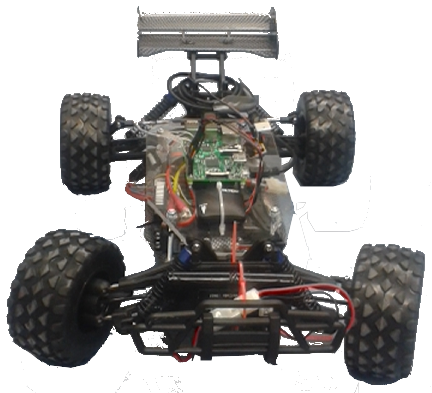
\includegraphics[width=.4\textwidth]{transparent_side1.png}
\end{center}
\vspace{-1cm}
\section{Milestones}

\begin{tabular}{ll}
\it{bis Weihnachten:}&
\bullet\ Auto Bausatz zusammenbauen\\
&
\bullet\ In RaspberryPi Programmierung einarbeiten\\
&\\
\it{bis Ende der Weihnachtsferien:}&
%\piccaption{Mini-Monstertruck}
%\parpic[r]{\includegraphics{truck.jpg}}
\bullet\ Auto steuern lernen (ohne GPS)\\
&\\
\it{bis Ende Januar:}&
\bullet\ GPS auslesen lernen\\
&\\
\it{bis Anfang Februar:}&
\bullet\ Navigationskonzept erarbeiten (ohne Hindernisse; Software)\\
&
\bullet\ GPS einbauen \& testen\\
&\\
\it{bis Anfang März:}&
\bullet\ Sensoren einbauen \& kalibrieren\\
&
\bullet\ Ausweich-Algorithmus entwickeln (Software)\\
&\\
\it{bis Mitte März:}&
\bullet\ Ausweichautomatik implementieren \& testen\\
&
\bullet\ Poster \& Präsentation erstellen
\end{tabular}
\vspace{-.25cm}
\section{Gruppenmitglieder}
\vspace{-.25cm}
\begin{multicols}{3}
\begin{center}
Philipp Gernandt\\
Master Physik 1. Semester\\
Gernandt@stud.uni-heidelberg.de\\
Maximilian Hartmann\\
Master Physik 3. Semester\\
maximilian.hartmann@stud.uni-heidelberg.de\\
Tobias Buck\\
Master Physik 3. Semester\\
Buck@stud.uni-heidelberg.de
\end{center}
\end{multicols}


\end{document}

